\chapter{\textbf{}} 	% titre "Annexe" pas nécessaire entre {} car apparaît une deuxième fois

\begin{center}
\textbf{Titre de l'article} \\
\textit{Journal} (Année), Volume (Issue): pages. \\
Auteurs 
\end{center}

\section{Titre}
\lipsum[1]

\FloatBarrier
\begin{landscape}
\pagestyle{empty} % enlever le numéro de page par défaut qui apparaîtra dans la marge de gauche 
\begin{figure}[htb]
%\captionsetup{format=hang,justification=raggedright,labelfont=bf, singlelinecheck = false, font=bf, labelsep=quad}
\centering
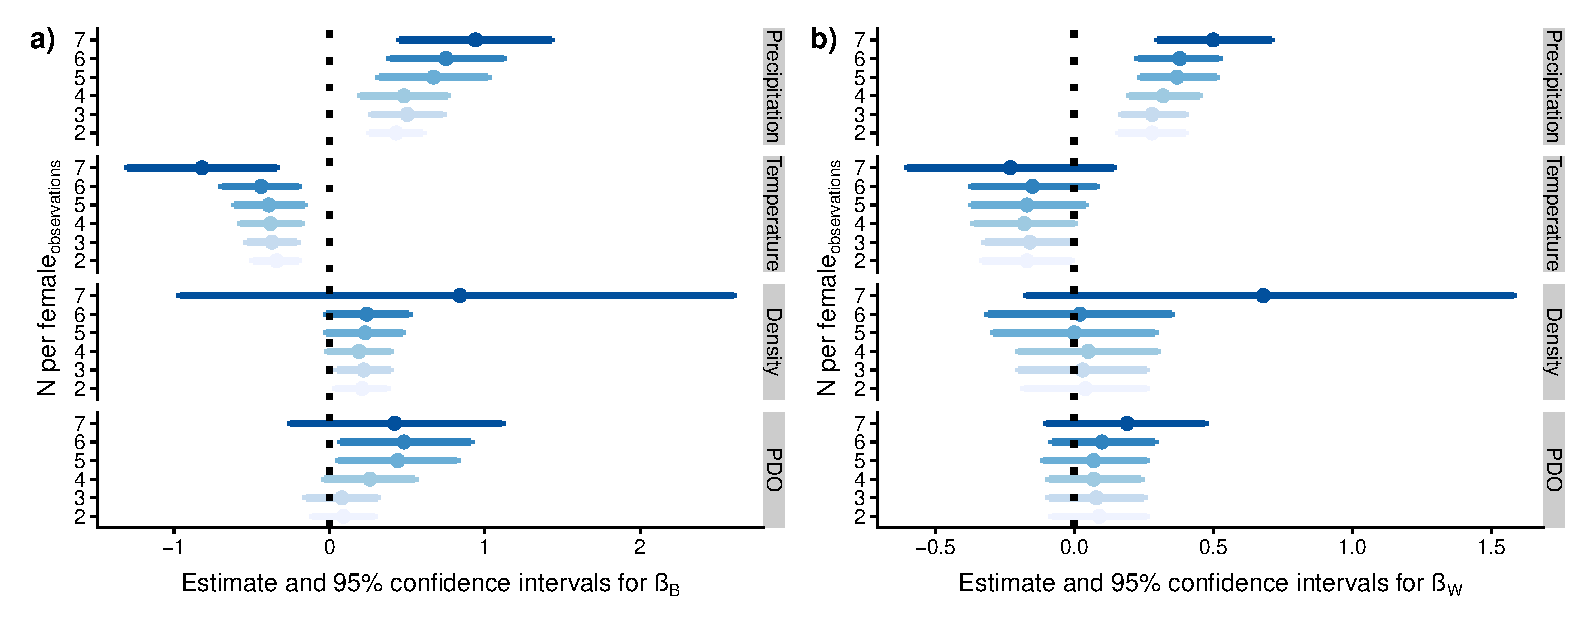
\includegraphics[width=\linewidth]{figs/annexe/ch2/ch2FigS1}
\caption[Titre de figure]{\label{ch2FigS1}Titre de figure\par{}
\smallskip		% saut de ligne entre titre et légende de figure
\normalfont{
Mean-centering was applied as suggested by \cite{Siepielski2017}}}. 
\end{figure}
\FloatBarrier
\end{landscape}

%-------------------BIBLIOGRAPHIE----------------------------
% assurez vous d’avoir un dossier avec vos listes de références par chapitre. C’est ici que chaque liste est intégrée au chapitre. 
% il faut la commande \bibliography ET \bibliographystyle pour que la liste par chapitre (avec différents styles) fonctionne. 

\singlespacing 
{\renewcommand{\bibname}{References}
\renewcommand{\bibsection}{\section{\bibname}}
\bibliography{bib/chapitre2}}
\bibliographystyle{styles/myBEAS} 
